\maketitle% this prints the handout title, author, and date

\begin{abstract}
\noindent
In this experiment, the barrier to rotation in \iupac{\N,\N-dimethylacetamide} can be determined by measuring changes in \NMR* line shapes as a function of temperature. This study is an example of dynamic NMR spectroscopy (spectroscopy on a changing system, as opposed to a static one).\thanks{Transcribed from \textcite{nibler14,gasparro77}.}
\end{abstract}

\section{Theory} % (fold)
\label{sec:theory}

\subsection{Magnetic Moments} % (fold)
\label{sub:magnetic_moments}

\begin{marginfigure}
  \centering
  \documentclass{standalone}
\usepackage{amsmath}
\usepackage{pgfplots}
\pgfplotsset{compat=1.16}
\usepgfplotslibrary{groupplots}
\usetikzlibrary{math}
\usetikzlibrary{calc}
\usetikzlibrary{arrows.meta}
\begin{document}

\pgfplotsset{
    width=0.95\textwidth,
    scale only axis,}
		
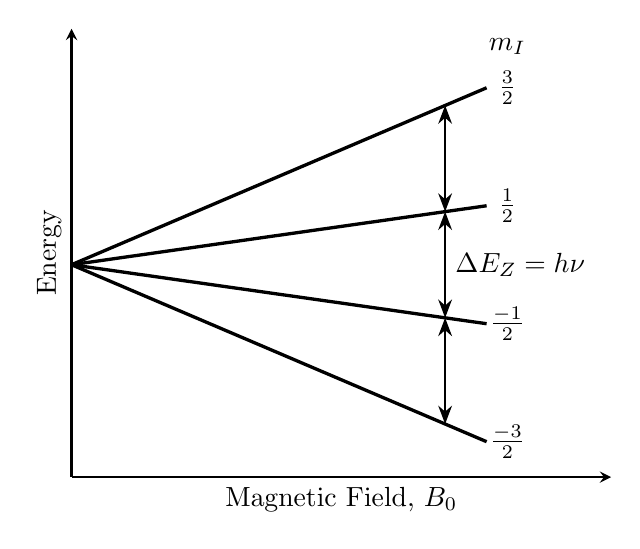
\begin{tikzpicture}
	\begin{axis}[
		axis lines = {left},
		smooth,
		thick,
		xlabel = {Magnetic Field, $B_0$}, 
		ylabel = Energy, 
		ticks = none,
		no markers, 
		xmin=0, xmax=13,
		ymin=-18, ymax=20,
		scale=1.0]

		\pgfplotsinvokeforeach{0,...,3}{
			\addplot [very thick, black, samples=50, domain=0:10] {(#1 - 3/2) * x};
			\node (#1) at (axis cs: {10.5},{10*(#1-3/2)}) {\(\frac{\pgfmathparse{int(2*#1-3)} \pgfmathresult}{2}\)};
		}

		% Annotation lines and arrows
		\pgfplotsinvokeforeach{0,...,2}{
			\draw[Stealth-Stealth] (axis cs: {9},{9*(#1-3/2)}) -- (axis cs: {9},{9*(#1-1/2)});
		}

		\node[right]	(Ez)	at	(axis cs: {9},{0})	[align=left]{$\Delta E_{\mathup{Z}} = h \nu$};
		\node (mS) at (axis cs: {10.5},{18.5}) {\(m_I\)};
	\end{axis}
\end{tikzpicture}	
\end{document}

  \caption{Energy levels and allowed transitions of a nucleus with \( I = 3/2 \) in a magnetic induction of magnitude \( B \).}
  \label{fig:quad_splitting}
\end{marginfigure}
The magnetic moment of a nucleus with nuclear spin quantum number \( I \) is 
\begin{equation}
	\mu = g_N \mu_N \sqrt{I \br{I+1}} \, ,
	\label{eq:mag_mom}
\end{equation}
where \( g_N \) is the nuclear \( g \) factor (\num{5.5856} for a proton) and \( \mu_N = e h / \br{4 \pi m_\mtext{p}} \) is the nuclear magneton.
Substitution of the charge \( e \) and mass of a proton, \( m_\mtext{p} \), gives the value of \qty{5.051e-27}{\joule\per\tesla} for \( \mu_N \). 
The symbol \( \mu_N \) is the unit of nuclear magnetic moment and is smaller than the electronic Bohr magneton (\( \mu_B \)) by the electron-to-proton mass ratio (\num{\sim1800}). 
\
The nuclear moment will interact with a local \emph{magnetic induction} (flux density)\sidenote{
	The vector quantity \( \vb{B} \) is called either the \emph{magnetic induction} or the \emph{magnetic flux density}, although the term \emph{magnetic field strength} is more commonly used.
	Unfortunately, the name \emph{magnetic field strength} was given to \( \vb{H} \) at a time when \( \vb{H} \) was considered to be the fundamental magnetic-field vector.
	It is now known that \( \vb{B} \) is the fundamental vector (analogous to \( \vb{E} \), the electric-field vector).
	To add to the confusion, \( \vb{B} = \vb{H} \) in a vacuum when CGS units are used.
	In the internationally-recognized SI system, \( \vb{B} = \mu_0 \vb{H} \) in a vacuum, and the vacuum permeability \( \mu_0 = \qty{4 \pi e-7}{\henry\per\m} \).
	In SI units, \( \vb{B} \) is expressed in tesla (\( \qty{1}{\tesla} = \qty{1}{\weber\per\meter\squared} = \qty{1e4}{\gauss}\)) and \( \vb{H} \) is expressed in \unit{\A\per\m}.
	In many texts, \( \vb{B} \) is loosely called the \emph{magnetic field}.
}, 
\( B_\mtext{loc} \), to cause an energy change (the Zeeman effect)
\begin{equation}
	E_\mtext{Zeeman} = -g_N \mu_N M_I B_\mtext{loc} \, .
	\label{eq:zeeman_energy}
\end{equation}
Here, \( M_I \) is the quantum number measuring the component of nuclear spin angular momentum (and magnetic moment) along the field direction, which can have values of \( -I, -I+1, \ldots, +I \). 
The effect of the field is thus to break the \( 2I + 1 \) degeneracy and to produce energy levels whose spacing increases linearly with \( B_\mtext{loc} \) (or \( B \)), as shown in \cref{fig:quad_splitting}. 
Transitions among these levels can be produced by electromagnetic radiation, provided that the selection rule \( \increment M_I = \pm 1 \) is satisfied. 
In this case, the resonant frequency is given by 
\begin{equation}
	\nu = \frac{\increment E_\mtext{Zeeman}}{h} = \frac{g_N\mu_N}{h} B_\mtext{loc}\, .
	\label{eq:res_freq}
\end{equation}
For protons, \( \nu = \num{4.26e7} \cdot B_\mtext{loc} \), where \( \nu \) is expressed in hertz and \( B_\mtext{loc} \) is expressed in tesla. For typical fields of \SIrange{1}{20}{\tesla}, \( \nu \) falls in the radio-frequency region (\SIrange{10}{1000}{\MHz}). 
In practice, values of \( B_0 \) (the external applied field) are chosen to fix \( \nu \) to some convenient value (e.g., \SIlist{400;600;800}{\MHz}). 

% subsection magnetic_moments (end)

\subsection{Chemical Shifts} % (fold)
\label{sub:chemical_shifts}

\Cref{eq:zeeman_energy} gives the energy energy levels of a nucleus in the presence of an external applied field. 
The term \( B_\mtext{loc} \) is the magnetic induction (\emph{local field}) at the nucleus. 

In general, the local induction, \( B_\mtext{loc} \), at the nucleus will differ from the externally applied induction, \( B_0 \), because of the magnetization, \( M \), that is induced by \( B_0 \):
\begin{equation}
	B_\mtext{loc} = B_0 + \mu_0 M = \br{1 + \chi} B \, ,
	\label{eq:b_loc}
\end{equation}
where \( \mu_0 \) is the vacuum permeability and \( \chi \) is the (dimensionless) volume susceptibility, the magnetic analog of dielectric polarizability. 

As most organic compounds are diamagnetic, only the diamagnetic contribution to the susceptibility is important in determining the resonance condition for a given nucleus. 
The diamagnetic contribution arises because the orbital motion of the electrons is altered by the presence of \( B_0 \) so that there is a net orbiting of electrons about the field lines. 
This circulating charge in turn generates a magnetic induction, \( B_d \), which is proportional and directly opposed to the external field, \( B_0 \). 
Thus, \( B_\mtext{loc} \) equals \( B_0 + B_d \), with
\begin{equation}
	B_d = \chi B_0 = -\sigma B_0 \, ,
	\label{eq:B_dia}
\end{equation}
where \( \sigma \) is a positive constant called the \emph{shielding constant}. 
The resonant frequency of nucleus \( i \) becomes 
\begin{equation}
	\nu_i = \frac{g_N \mu_N}{h} B_{i, \mtext{loc}} = \frac{g_N \mu_N}{h} B_0 \br{1 - \sigma} \, .
	\label{eq:chem_shift}
\end{equation} 
The diamagnetic shielding constant, \( \sigma \), is generally quite small (\num{\sim e-5}) and increases as the electron density around the nucleus is increased. 
Changes in the local induction (\( B_\mtext{loc} = B_0 \br{1 - \sigma} \)), and thus changes in \( \nu \), of a few parts per million (\unit{\ppm}) are typical when the chemical environment about a nucleus is changed. 
The chemical shift in \unit{ppm} of a nucleus \( i \) relative to a reference nucleus \( r \) is defined by 
\begin{equation}
	\delta_{i} \equiv 
		\frac{\nu_{i}-\nu_\mtext{ref}}{\nu_\mtext{ref}} \times 10^6 = 
		\frac{\sigma_\mtext{ref} - \sigma_i}{1 - \sigma_\mtext{ref}} \times 10^6 \simeq 
		\br{\sigma_\mtext{ref} - \sigma_i} \times 10^6 \, .
		\label{eq:chem_shift_delta}
\end{equation}
Here, the definition is based on the resonant frequencies for a fixed external induction (field), \( B_0 \). 

\begin{figure}[htb]
  \centering
  \documentclass{standalone}

\usetikzlibrary{decorations.markings}

\begin{document}
  
\setchemfig{atom style={scale=1}}
\begin{tikzpicture}[
      decoration={
          markings,
          mark=at position 0.27 with {\arrow{stealth}},
          mark=at position 0.77 with {\arrow{stealth}}
      }
  ]

  %%% Proton shielding
  \begin{scope}[shift={(-3,0)}]
            
      %% Back bond current ring
      \draw [blue, thick] (1,0) arc (0:180:1 and 0.35);
      %% small template ring
      % \draw [gray, postaction={decorate}] (1.3,0) ellipse (0.8 and 1.2);
      %% large template ring
      % \draw [gray, postaction={decorate}] (1.85,0) ellipse (1.6 and 2.4);
      %% Outer field rings
      \draw [red, postaction={decorate}] 
          (2,2) arc (90:270:2);
      \draw [red, postaction={decorate}] 
          (-2,2) arc (90:-90:2);
      
      % \draw [black, postaction={decorate}]
%             (-2.09,0.15) arc (173:0:0.8 and 1.2);
%         \draw [black, postaction={decorate}]
%             (-0.58,-.5) arc (335:187:0.8 and 1.2);
      %% Middle field rings
      % \draw [gray] (0.25,0) arc (-180:180:1.5);
      \draw [red, postaction={decorate}] 
          (2,1.475) arc (80:280:1.5);
      \draw [red, postaction={decorate}] 
          (-2,1.475) arc (100:-100:1.5);
      %% Inner field rings
      \draw [red, postaction={decorate}] 
          (0.5,0) arc (-180:180:0.75);
      \draw [red, postaction={decorate}] 
          (-0.5,0) arc (360:0:0.75);
          
      % Proton
      \draw [black, thick,fill=white] (0,0) circle (0.6);
      
      %% Bond current ring
      \draw [blue, thick, postaction={decorate}] 
          (-.71,.25) arc (135:405:1 and 0.35);
      
      %% External magnetic field
      \draw [black,line width=4pt,arrows={-Triangle[angle=45:15pt]}] 
          (0,-2.5) node[above right=-1pt] {\(B_0\)} node[below] {(a)} -- (0,-0.75);
  \end{scope}
      
  \begin{scope}[shift={(3,0)}]
      %% Benzene molecule
      \node at 
          (0,0) {\chemfig[cram width=2pt]{
              H-?<[7,0.7]-[,,,, line width=2pt]>[1,0.7](-H)-[3,0.7]-[4]?
          }};
      %% Bond current ring
      \draw [blue, thick, postaction={decorate}] 
          (0,0) ellipse (0.7 and 0.35);
      
      %% small template ring
      % \draw [gray, postaction={decorate}] (1.3,0) ellipse (0.8 and 1.2);
      %% large template ring
      % \draw [gray, postaction={decorate}] (1.85,0) ellipse (1.6 and 2.4);
      %% Outer field rings
      \draw [red, postaction={decorate}] 
          (2.09,0.15) arc (7:180:0.8 and 1.2);
      \draw [red, postaction={decorate}] 
          (0.58,-.5) arc (-155:-7:0.8 and 1.2);
      \draw [red, postaction={decorate}] 
          (-2.09,0.15) arc (173:0:0.8 and 1.2);
      \draw [red, postaction={decorate}] 
          (-0.58,-.5) arc (335:187:0.8 and 1.2);
      %% Inner field rings
      \draw [red, postaction={decorate}] 
          (1.05,2.08) arc (120:180:1.6 and 2.4);
      \draw [red, postaction={decorate}] 
          (0.285,-0.50) arc (192:240:1.6 and 2.4);
      \draw [red, postaction={decorate}] 
          (-1.05,2.08) arc (60:0:1.6 and 2.4);
      \draw [red, postaction={decorate}] 
          (-0.285,-0.50) arc (348:300:1.6 and 2.4);
      
      %% External magnetic field
      \draw [black,line width=4pt,arrows={-Triangle[angle=45:15pt]}] 
          (0,-2.5) node[above right=-1pt] {\(B_0\)} node[below] {(b)} -- (0,-0.75);
  \end{scope}
  
  \begin{scope}[node distance=3mm]
      \node[text width=2.2cm,align=left, node font=\small] (a) at (0.5,-2.5) {Field produced by electron\\ circulation};
      \node[text width=2.0cm,align=left, node font=\small] (b) at (0.4,2.2) {Electron\\ circulation\\ induced by\\ applied field};
      
      \draw[-Stealth,thick] (b) -- (-2, 0.15);
      \draw[-Stealth,thick] (b) -- (2.3, 0.15);
      \draw[-Stealth,thick] (a) -- (-1.3, -0.7);
      \draw[-Stealth,thick] (a) -- (1.3, -1.2);

  \end{scope}
\end{tikzpicture}
\setchemfig{atom style={scale=0.80}}

\end{document}


  \caption{Shielding and deshielding of protons: (a) shielding of a proton due to induced diamagnetic electron circulation; (b) deshielding of protons in benzene due to aromatic ring currents.}
  \label{fig:shielding}
\end{figure}
  
Tetramethylsilane (TMS) is usually used as the proton reference, since it is chemically inert and its 12 equivalent protons give a single transition at a frequency \( \nu_\mtext{ref} \), lower than the frequency \( \nu_i \) found in most organic compounds. 
Thus, \( \delta \) is generally positive and increases when substituents are added that attract electrons and thereby reduce the shielding about the proton. 
This shielding arises because the electrons near the proton are induced to circulate by the applied field \( B_0 \), shown in \cref{fig:shielding}. 
This electron current produces a secondary field that \emph{opposes} the external field and thus reduces the local field at the nucleus. 
As a result, resonance at a fixed field, such as \qty{9.4}{\tesla}, requires a higher frequency for protons with greater shielding. 
This shielding effect is generally restricted to electrons localized on the nucleus of interest, since random tumbling of molecules causes the effect of secondary fields due to electrons associated with neighboring nuclei to average to zero. 
Nuclei such as \ch{^{19}F}, \ch{^{13}C}, and \ch{^{11}B} have more local electrons than hydrogen, hence their chemical shift ranges are much larger. 

\begin{table}[ht]
	\centering
	\begin{tabular}{lS@{\hspace{3em}}lS} 
		\toprule
		\headercell{\ch{CH3} protons}	&	\headercell{Acetylenic protons} \\
		\ch{(CH3)4Si}	&	0.0	&	\ch{HOCH2C+CH}	& 2.33 \\
		\ch{(CH3)4C} & 0.92 & \ch{ClCH2C+CH} & 2.40 \\
		\ch{CH3CH2OH} & 1.17 & \ch{CH2COC+CH} & 3.17\\
		\ch{CH3COCH3} & 2.07 & \headercell{Olefinic protons}\\
		\ch{CH3OH} & 3.38 & \ch{(CH3)2C=CH2} & 4.6 \\
		\ch{CH3F} & 4.30 & \iupac{Cyclohexene} & 5.57 \\
		\headercell{\ch{CH2} protons} & \ch{CH2CH=CHCHO} & 6.05 \\
		\iupac{Cyclopropane} & 0.22 & \ch{Cl2C=CHCl} & 6.45 \\
		\ch{CH3(CH2)4CH3} & 1.25 & \headercell{Aromatic protons} \\
		\ch{(CH3CH2)2CO} & 2.39 & \iupac{Benzene} & 7.27 \\
		\ch{CH3COCH2COOCH3} & 3.48 & \ch{C6H5CN} & 7.54 \\
		\ch{CH3CH2OH} & 3.59 & \iupac{Naphthalene} & 7.73 \\
		\headercell{\ch{CH} protons} & \iupac{\a-Pyridine} & 8.50 \\
		\iupac{Bicyclo[2.2.1]heptane} & 2.19 & \headercell{Aldehydic protons} \\
		\iupac{Chlorocyclopropane} & 2.95 & \ch{CH3OCHO} & 8.03 \\
		\ch{(CH3)2CHOH} & 3.95 & \ch{CH3CHO} & 9.72 \\
		\ch{(CH3)2CHBr} & 4.17 & \ch{C6H5CHO} & 9.96 \\
		\bottomrule
	\end{tabular}
	\caption{Typical proton chemical shifts $\delta$ (\unit{ppm}).}
	\label{tab:chem_shifts}
\end{table}

Long-range \emph{deshielding} can occur in aromatic and other molecules with delocalized \( \pi \) electrons. 
For example, when the plane of the benzene molecule is oriented perpendicular to \( B_0 \), circulation of the \( \pi \) electrons produces a ring current, illustrated in \cref{fig:shielding}. 
This ring current induces a secondary field at the protons that is aligned \emph{parallel} to \( B_0 \) and results in a higher local field for the protons. 
This induced field changes with benzene orientation, but does not average to zero, since it is not spherically symmetric. 
Because of this net deshielding effect, the resonance of the benzene protons occurs at a relatively high frequency. 
The proton chemical shift \( \delta  \) for benzene is \qty{7.27}{\ppm}, much higher in frequency from the value \( \delta = \qty{1.43}{\ppm} \) that is observed for cyclohexane, in which ring currents do not occur. 
Similar deshielding values of \( \delta \) for different functional groups are shown in \cref{tab:chem_shifts}, and additional values are available in refs.~\autocite{davis1965advanced,pople1959nmr,silverstein2005spec,sdbs2020,aldrich1993nmr}.
Although the resonances change somewhat for different compounds, the range for a given functional group is usually small and \( \delta \) values are widely used for structural characterization in organic chemistry. 


% subsection chemical_shifts (end)

\subsection{Spin--Spin Splitting} % (fold)
\label{sub:spin_spin_splitting}

High-resolution NMR spectra of most organic compounds reveal more complicated spectra than those predicted by \cref{eq:chem_shift}, with transitions often appearing as multiplets.
Such \emph{spin--spin splitting patterns} arise because the magnetic moments of one nucleus (A) can interact with that of a nearby nucleus (B), causing a small energy shift up or down depending on the relative orientations of the two moments. 
The energy levels of nucleus A then have the form 
\begin{equation}
	E_\mtext{A} = -g_{N_\mtext{A}} \mu_N M_{I_\mtext{A}} \br{1-\sigma_\mtext{A}} B_0
		+ h J_\mtext{AB} M_{I_\mtext{A}} M_{I_\mtext{B}}
	\label{eq:j_coupling}
\end{equation}
and there is a similar expression for \( E_\mtext{B} \). 
The spin--spin interaction is characterized by the coupling constant \( J_\mtext{AB} \), and the effect is to split the energy levels in the manner illustrated for acetaldehyde in \cref{fig:spin_splitting}. 
It is apparent from this diagram that the external field \( B_0 \) does not affect the small spin--spin splitting that is characterized by the coupling constant \( J \). 
The quantity \( J \) is a measure of the strength of the pairwise interaction of the spin nucleus A with the spin of nucleus B. 
Since there are only proton--proton interactions in acetaldehyde, the same splitting occurs for both \ch{CH} and \ch{CH3} resonances. 

\begin{figure}[htb]
  \centering
  \documentclass{standalone}
% %% Header file cloned from https://github.com/wickles/latex-base

%%%%%%%%%%%%%%%%%%
%% CONTENTS
%%%%%%%%%%%%%%%%%%
% To-do / issues
% Packages
% Commands
% Special Symbols
% Environments
% Notes
%%%%%%%%%%%%%%%%%%
%%%%%%%%%%%%%%%%%%



%%%%%%%%%%%%%%%%%%
%% TO-DO / ISSUES
%%%%%%%%%%%%%%%%%%

% Fix header format in tufte-latex (bad spacing, no small-caps font in Charter). 
% Replace \Molar unit, check for \textsc




%%%%%%%%%%%%%%%%%%
%% PACKAGES
%%%%%%%%%%%%%%%%%%


%% debugging / diagnostics
\RequirePackage[l2tabu,orthodox]{nag} % nags user about obsolete and improper syntax

\usepackage{xparse} % provides high-level interface for producing document-level commands
	% via \[Declare/New/Renew/Provide/etc]DocumentCommand
	% allows for more than one optional argument in commands

\usepackage{ifdraft}

%% fonts and encoding 

\newcommand{\textools}[2][5]{%
	\begingroup\addfontfeatures{LetterSpace=#1}#2\endgroup
	}
\renewcommand{\allcapsspacing}[1]{\textools[15]{#1}}
\renewcommand{\smallcapsspacing}[1]{\textools[10]{#1}}
\renewcommand{\allcaps}[1]{\textools[15]{\MakeTextUppercase{#1}}}
\renewcommand{\smallcaps}[1]{\textit{#1}} 
	% Version of Charter font included with macOS 13 doesn't work with \textsc
	% It uses individual smallcaps glyphs instead. 
% \renewcommand{\textsc}[1]{\smallcapsspacing{\textsmallcaps{#1}}}

%% font packages -- load fontspec, then select fonts and features. 

\usepackage{fontspec}
\usepackage[math-style=ISO,mathrm=sym]{unicode-math} 
\ifdraft{}{
	\setmainfont{Charter}
	\setmathfont{STIX Two Math}
	\setmonofont{Consolas}
}


% standard and structural packages

\usepackage{bm} % provides \bm command for robustly bolding math characters
\usepackage{microtype} % improves kerning in certain cases. 
	% recommended to disable protrusion in table of contents!

%% Latex interface 

\usepackage{letltxmacro} % provides \LetLtxMacro command for correct renaming of commands
\usepackage{etoolbox} % provides many useful programming tools, 
	% e.g. \ifdefempty{cs}{true}{false}



%% media interface

\usepackage{graphicx} % support the \includegraphics command and options
\usepackage{subfig} % Support for subfigures and subcaptions
	\captionsetup[subfloat]{position=bottom}
\usepackage{pgfplots} % for plotting in tikzpicture environment
	\pgfplotsset{compat=1.16} % required to select newest version
\usepackage{tikzscale} % allows \includegraphics{*.tikz} and scaling of TiKZ images


%% math interface

\usepackage{amsmath} % for nice math commands and environments
\usepackage{mathtools} % extends amsmath with bug fixes and useful commands, e.g.
	% \shortintertext for short interjections in align environment,
	% \prescript{t}{b}{X} for simple, nicely aligned math pre-(super/sub)scripts
	% \Aboxed{...} for boxing full lines in 'align' environment
\usepackage{derivative} % provides \odv, \pdv, \odif, \pdif
\usepackage{bropd} % provides \br command which simplifies nesting of bracketed terms 
	% e.g. \br{\br{x-a}^2+\br{y-b}^2} produces \left[ \left( x-a \right)^2 + \left( y-b \right)^2 \right]
\usepackage{array} % improves array support, esp. in tabular env. 
	% see also xtab.sty
\usepackage{booktabs} % allows for improved spacing in tabular env. 
	% use \toprule, \*midrule, \bottomrule instead of \hline


%% Science and programming packages
\usepackage{fvextra} % for verbatim and comment environments with \Verb
\usepackage{chemmacros} % for writing chemical formulas with \ch, e.g. \ch{AgCl2-} or \ch{^{227}_{90}Th+}
	\usechemmodule{
		spectroscopy, % loads formula and siunitx modules, provides \NMR command.  
	    thermodynamics, % provides state variables and equations
    	units, % provides \[mM]olar, \Torr, \atm, \cal, \cmc, \MolMass
		} % also loads siunitx and chemformula
	\sisetup{% siunit package options
		per-mode = symbol,%
		inter-unit-product=\ensuremath{{}\!\cdot\!{}},%
		separate-uncertainty,%
		multi-part-units = single,%
		retain-explicit-plus,%
		list-final-separator={, and },%
		math-celsius = °\text{C}, % for temperatures
		text-celsius = °C,
		math-degree = °, % for angles
		text-degree = °,%
		input-digits = 0123456789 \pi \mitpi% necessary to use \pi in SI entries, affects rounding of digits.
		}%
	\DeclareSIUnit\ppm{ppm}
	\DeclareSIUnit\angstrom{\text{Å}} % Symbol doesn't exist in STIXTwoMath, need to force text font. 
	\DeclareSIUnit\wn{cm^{-1}}
	

%% misc packages

\usepackage{framed} % provides boxed 'framed' environment for easily boxing text 
\usepackage{tcolorbox}
	\tcbuselibrary{skins, breakable, xparse, minted}
	% provides fancier boxes than regular \makebox, \fbox, etc.
	% e.g. \doublebox, \ovalbox, \shadowbox
	% Can use `\tcbuselibrary{listings}` to use the listings library, 
		% doesn't require a language to be defined. 
\usepackage{empheq} % provides 'empheq' environment 
	% for improved control over shape, size, color of framed boxes, e.g. 
\newcommand{\boxedeq}[2]{
	\begin{empheq}[box={\fboxsep=6pt\fbox}]{align}\label{#1}#2\end{empheq}
}
\newcommand{\coloredeq}[2]{
	\begin{empheq}[box=\colorbox{lightgreen}]{align}\label{#1}#2\end{empheq}
}


%% document interface 

\usepackage{footnote} % 
\usepackage{hyperref} % adds hyperlinks and outline to PDF documents
	\hypersetup{%
		pdfencoding=auto,%
		psdextra,%
		pdfusetitle,%
		colorlinks=true,%
		linkcolor=BrickRed, %
		citecolor=Green, %
		filecolor=Mulberry, %
		urlcolor=NavyBlue, %
		menucolor=BrickRed, %
		runcolor=Mulberry, %
		linkbordercolor=BrickRed, %
		citebordercolor=Green, %
		filebordercolor=Mulberry, %
		urlbordercolor=NavyBlue, %
		menubordercolor=BrickRed, %
		runbordercolor=Mulberry %
		} %
	% options enable enhanced unicode and math support in PDF outlines [causes conflict with \C command?]
\usepackage{cleveref} % provides \cref command which inserts contextually correct word in front of ref.
	% e.g. \cref{eq:myeq} --> Equation 1.2, or so
\usepackage{bookmark} % improves package hyperref's bookmarking. 
	% properties such as style and color can be set. Generates bookmarks in first run. 


%% load later packages
\usepackage[textsize=footnotesize]{todonotes}



%%%%%%%%%%%%%%%%%%
%% COMMANDS
%%%%%%%%%%%%%%%%%%

\newcommand{\mtext}[1]{{\mathup{#1}}}
\DeclareMathOperator{\sgn}{sgn}
\DeclareMathOperator{\erf}{erf}
\DeclareMathOperator{\erfc}{erfc}
\DeclareMathOperator{\GammaFunc}{\symup{\Gamma}}
\DeclareMathOperator{\laplacian}{\nabla^2}
\DeclarePairedDelimiter\abs{\lvert}{\rvert}
\newcommand{\vb}[1]{\symbfit{#1}}

%% pre-defined colors
% standard: black, blue, brown, cyan, darkgray, gray, green, lightgray, lime, magenta, olive, orange, pink, purple, red, teal, violet, white, yellow
%
% dvips: Apricot, Aquamarine, Bittersweet, Black, Blue, BlueGreen, BlueViolet, BrickRed, Brown, BurntOrange, CadetBlue, CarnationPink, Cerulean, CornflowerBlue, Cyan, Dandelion, DarkOrchid, Emerald, ForestGreen, Fuchsia, Goldenrod, Gray, Green, GreenYellow, JungleGreen, Lavender, LimeGreen, Magenta, Mahogany, Maroon, Melon, MidnightBlue, Mulberry, NavyBlue, OliveGreen, Orange, OrangeRed, Orchid, Peach, Periwinkle, PineGreen, Plum, ProcessBlue, Purple, RawSienna, Red, RedOrange, RedViolet, Rhodamine, RoyalBlue, RoyalPurple, RubineRed, Salmon, SeaGreen, Sepia, SkyBlue, SpringGreen, Tan, TealBlue, Thistle, Turquoise, Violet, VioletRed, White, WildStrawberry, Yellow, YellowGreen, YellowOrange

\usepackage{pgfplots}
\pgfplotsset{compat=newest}
\usepgfplotslibrary{groupplots}
\usetikzlibrary{math}
\usetikzlibrary{calc}
\usepackage{siunitx,chemmacros}
\begin{document}

%% Create single x label for grouped plots  
\makeatletter
\pgfplotsset{
    groupplot xlabel/.initial={},
    every groupplot x label/.style={
        at={
            ($(
                {\pgfplots@group@name\space c1r\pgfplots@group@rows.west} |- 
                {\pgfplots@group@name\space c1r\pgfplots@group@rows.outer south}
            )!0.5!(
                {\pgfplots@group@name\space c\pgfplots@group@columns r\pgfplots@group@rows.east} |- 
                {\pgfplots@group@name\space c\pgfplots@group@columns r\pgfplots@group@rows.outer south}
            ) -(0.0,0.5)$)
            },
        anchor=north,
        align=center,
    },
    groupplot ylabel/.initial={},
    every groupplot y label/.style={
            rotate=90,
        at={
            ($(
                {\pgfplots@group@name\space c1r1.north} -|
                {\pgfplots@group@name\space c1r1.outer west}
            )!0.5!(
                {\pgfplots@group@name\space c1r\pgfplots@group@rows.south} -|
                {\pgfplots@group@name\space c1r\pgfplots@group@rows.outer west}
            )$)
        },
        anchor=south
    },
    execute at end groupplot/.code={%
      \node [/pgfplots/every groupplot x label]
        {\pgfkeysvalueof{/pgfplots/groupplot xlabel}};  
      \node [/pgfplots/every groupplot y label]
        {\pgfkeysvalueof{/pgfplots/groupplot ylabel}};
    }
}

\def\endpgfplots@environment@groupplot{%
    \endpgfplots@environment@opt%
    \pgfkeys{/pgfplots/execute at end groupplot}%
    \endgroup%
}
\makeatother

%% Create style for NMR spectra (color cycle, x-axis label, tick precision)
\pgfplotsset{
  nmr/.style={
  % Using a cycle list just altering colour means that there are no
  % marks: that is normal for this sort of plot.
  cycle list name=color list, 
  % Ensure that the x-axis values always have the same number of 
  % decimal places, to avoid e.g. "1" but "1.2".
  every x tick label/.append style={ 
    /pgf/number format/.cd,
     precision=2, 
     fixed,
     zerofill,
  },
  % The labels apply to all plots of this type.
  % Notice that in this case the zero is TMS, but that
  % will depend on the experiment.
  % xlabel = $\delta \, (\si{ppm})$,
  },
}

% Not everyone likes the 'axis box' effect which is the pgfplots default.
% Here, we'll set up to use 'Tufte-like' settings: see
% https://www.tug.org/members/TUGboat/tb34-2/tb107dugge.pdf for more on
% this.
% \makeatletter
\pgfplotsset{
  tufte axes/.style={
	% after end axis/.code={
    % \draw ({rel axis cs:0,0} -| {axis cs:\pgfplots@data@xmin,0})
    %   -- ({rel axis cs:0,0}  -| {axis cs:\pgfplots@data@xmax,0});
    % },
	axis x line = bottom,
  axis y line = none,
  every inner x axis line/.append style={-|},
  tick align = outside,
  tick pos   = left,
	ytick			 = \empty,
  x dir			 = reverse,
  }
}
% \makeatother

\pgfplotsset{
    width=0.95\textwidth,
    height=1.4\textwidth,
    scale only axis,}
    
\begin{tikzpicture}
  \begin{groupplot}[group style={
      group size=2 by 1,
      xticklabels at=edge bottom,
      horizontal sep=0pt,
      every plot/.style={nmr}
    },
    groupplot xlabel={
      $\delta \, (\si{ppm})$ \\ $\Leftarrow \nu, \, B_\textup{loc}$},
    ymin=-0.08, ymax=6.75,
  ]
  
  \nextgroupplot[
    xmin=9.67,xmax=9.87,
    % ymin=-0.08, ymax=1.8,
    axis x line   = bottom,
    axis y line   = none,
    every inner x axis line/.append style={-|},
    tick align    = outside,
    tick pos      = left,
    ytick     = \empty,
    x dir      = reverse,
    axis x discontinuity=crunch,
    width=0.55\textwidth,
  ]
    
    \tikzmath{
      \pkctr=9.789;
      \lvctr=2.5;
      \lvwidth=0.02/2;
      \lvscale=\pkctr;
      \jCHO=2.9/100.0;
      %
      \pkcta=\pkctr+(3/2)*\jCHO;
      \pkctb=\pkctr+(1/2)*\jCHO;
      \pkctc=\pkctr-(1/2)*\jCHO;
      \pkctd=\pkctr-(3/2)*\jCHO;
      %
      \lev1=\lvctr-1/2*(0.2)*\lvscale;
      \lev2=\lvctr+1/2*(0.2)*\lvscale;
      %
      \levag=\lvctr-1/2*(\pkcta-\pkctr+.2)*\lvscale;
      \levae=\lvctr+1/2*(\pkcta-\pkctr+.2)*\lvscale;
      \aleft=\pkcta+\lvwidth;
      \aright=\pkcta-\lvwidth;
      %
      \levbg=\lvctr-1/2*(\pkctb-\pkctr+.2)*\lvscale;
      \levbe=\lvctr+1/2*(\pkctb-\pkctr+.2)*\lvscale;
      \bleft=\pkctb+\lvwidth;
      \bright=\pkctb-\lvwidth;
      %
      \levcg=\lvctr-1/2*(\pkctc-\pkctr+.2)*\lvscale;
      \levce=\lvctr+1/2*(\pkctc-\pkctr+.2)*\lvscale;
      \cleft=\pkctc+\lvwidth;
      \cright=\pkctc-\lvwidth;
      %
      \levdg=\lvctr-1/2*(\pkctd-\pkctr+.2)*\lvscale;
      \levde=\lvctr+1/2*(\pkctd-\pkctr+.2)*\lvscale;
      \dleft=\pkctd+\lvwidth;
      \dright=\pkctd-\lvwidth;
    }
    
    {\addplot table from {Figures/CH3CHO_nmr_simsc2.dat};
      \node (fragment) at (\pkctr,5.0) {\ch{-CHO}};
      \node[align=center,left=-4pt] (CHO) at (\aleft,4.5) [red]{\ch{CHO}\\spin};
      \node[align=center] (CH3) at (\pkctr,4.5) [blue]{\ch{CH3}\\spins};
      \coordinate (01) at (\dright,\lev1);
      \coordinate (02) at (\aleft,\lev1);
      \coordinate (11) at (\dright,\lev2);
      \coordinate (12) at (\aleft,\lev2);
      \coordinate (Ag1) at (\aright,\levag);
      \coordinate (Ag2) at (\aleft,\levag);
      \coordinate (Ag3) at (\pkcta, \levag);
      \coordinate (Ae1) at (\aright,\levae);
      \coordinate (Ae2) at (\aleft,\levae);
      \coordinate (Ae3) at (\pkcta, \levae);
      \coordinate (Bg1) at (\bright,\levbg);
      \coordinate (Bg2) at (\bleft,\levbg);
      \coordinate (Bg3) at (\pkctb, \levbg);
      \coordinate (Be1) at (\bright,\levbe);
      \coordinate (Be2) at (\bleft,\levbe);
      \coordinate (Be3) at (\pkctb, \levbe);
      \coordinate (Cg1) at (\cright,\levcg);
      \coordinate (Cg2) at (\cleft,\levcg);
      \coordinate (Cg3) at (\pkctc, \levcg);
      \coordinate (Ce1) at (\cright,\levce);
      \coordinate (Ce2) at (\cleft,\levce);
      \coordinate (Ce3) at (\pkctc, \levce);
      \coordinate (Dg1) at (\dright,\levdg);
      \coordinate (Dg2) at (\dleft,\levdg);
      \coordinate (Dg3) at (\pkctd, \levdg);
      \coordinate (De1) at (\dright,\levde);
      \coordinate (De2) at (\dleft,\levde);
      \coordinate (De3) at (\pkctd, \levde);
    };
    \begin{scope}[thick] 
      \draw[thin,dashed] (01) -- (02) node[left=1pt] 
        [red]{$\uparrow$};
      \draw[thin,dashed] (11) -- (12) node[left=1pt] 
        [red]{$\downarrow$};     
      \draw (Ag1) -- (Ag2);
      \draw (Ae1) -- (Ae2);
      \draw[-Stealth] (Ag3) -- (Ae3) node[above] 
        [blue]{$\downarrow\downarrow\downarrow$};
      \draw (Bg1) -- (Bg2);
      \draw (Be1) -- (Be2);
      \draw[-Stealth] (Bg3) -- (Be3) node[above] 
        [align=center,blue]{ 
          $\downarrow\downarrow\uparrow$ \\
          $\downarrow\uparrow\downarrow$ \\
          $\uparrow\downarrow\downarrow$};
      \draw (Cg1) -- (Cg2);
      \draw (Ce1) -- (Ce2);
      \draw[-Stealth] (Cg3) -- (Ce3) node[above] 
        [align=center,blue]{ 
          $\downarrow\uparrow\uparrow$ \\
          $\uparrow\downarrow\uparrow$ \\
          $\uparrow\uparrow\downarrow$};
      \draw (Dg1) -- (Dg2);
      \draw (De1) -- (De2);
      \draw[-Stealth] (Dg3) -- (De3) node[above] 
        [blue]{$\uparrow\uparrow\uparrow$};
    \end{scope}

  \nextgroupplot[
    xmin=2.15,xmax=2.26,
    % ymin=-0.08, ymax=1.8,
  	axis x line = bottom,
	  axis y line = none,
    x axis line style={|-},
    tick align      = outside,
    tick pos        = left,
  	ytick						= \empty,
	  x dir						= reverse,
    width=0.40\textwidth,]
    
    \tikzmath{
      \pkctr=2.206;
      \lvctr=2.5;
      \lvwidth=0.02/2;
      \lvscale=\pkctr;
      \jCHO=2.9/100.0;
      %
      \pkcta=\pkctr+(1/2)*\jCHO;
      \pkctb=\pkctr-(1/2)*\jCHO;
      %
      \lev1=\lvctr-3/2*(.25)*\lvscale;
      \lev2=\lvctr-1/2*(.25)*\lvscale;
      \lev3=\lvctr+1/2*(.25)*\lvscale;
      \lev4=\lvctr+3/2*(.25)*\lvscale;
      %
      \leva1=\lvctr-3/2*(\pkcta-\pkctr+.25)*\lvscale;
      \leva2=\lvctr-1/2*(\pkcta-\pkctr+.25)*\lvscale;
      \leva3=\lvctr+1/2*(\pkcta-\pkctr+.25)*\lvscale;
      \leva4=\lvctr+3/2*(\pkcta-\pkctr+.25)*\lvscale;
      \aleft=\pkcta+\lvwidth;
      \aright=\pkcta-\lvwidth;
      %
      \levb1=\lvctr-3/2*(\pkctb-\pkctr+.25)*\lvscale;
      \levb2=\lvctr-1/2*(\pkctb-\pkctr+.25)*\lvscale;
      \levb3=\lvctr+1/2*(\pkctb-\pkctr+.25)*\lvscale;
      \levb4=\lvctr+3/2*(\pkctb-\pkctr+.25)*\lvscale;
      \bleft=\pkctb+\lvwidth;
      \bright=\pkctb-\lvwidth;
    }
    
    {\addplot table from {Figures/CH3CHO_nmr_simsc1.dat};
      \node (fragment) at (\pkctr,5.0) {\ch{-CH3}};
      \node[align=center,left=-2pt] (CH3) at (\aleft,4.0) 
        [red]{\ch{CH3}\\spins};
      \node[align=center] (CHO) at (\pkctr,4.0) [blue]{\ch{CHO}\\spin};
      \coordinate (011) at (\bright,\lev1);
      \coordinate (012) at (\aleft,\lev1);
      \coordinate (021) at (\bright,\lev2);
      \coordinate (022) at (\aleft,\lev2);
      \coordinate (031) at (\bright,\lev3);
      \coordinate (032) at (\aleft,\lev3);
      \coordinate (041) at (\bright,\lev4);
      \coordinate (042) at (\aleft,\lev4);
      \coordinate (A11) at (\aright,\leva1);
      \coordinate (A12) at (\aleft,\leva1);
      \coordinate (A13) at (\pkcta, \leva1);
      \coordinate (A21) at (\aright,\leva2);
      \coordinate (A22) at (\aleft,\leva2);
      \coordinate (A23) at (\pkcta, \leva2);
      \coordinate (A31) at (\aright,\leva3);
      \coordinate (A32) at (\aleft,\leva3);
      \coordinate (A33) at (\pkcta, \leva3);
      \coordinate (A41) at (\aright,\leva4);
      \coordinate (A42) at (\aleft,\leva4);
      \coordinate (A43) at (\pkcta, \leva4);
      \coordinate (B11) at (\bright,\levb1);
      \coordinate (B12) at (\bleft,\levb1);
      \coordinate (B13) at (\pkctb, \levb1);
      \coordinate (B21) at (\bright,\levb2);
      \coordinate (B22) at (\bleft,\levb2);
      \coordinate (B23) at (\pkctb, \levb2);
      \coordinate (B31) at (\bright,\levb3);
      \coordinate (B32) at (\bleft,\levb3);
      \coordinate (B33) at (\pkctb, \levb3);
      \coordinate (B41) at (\bright,\levb4);
      \coordinate (B42) at (\bleft,\levb4);
      \coordinate (B43) at (\pkctb, \levb4);
    };
    \begin{scope}[thick] 
      \draw[dashed,thin] (011) -- (012) node[left=1pt] 
        [red]{$\uparrow\uparrow\uparrow$};
      \draw[dashed,thin] (021) -- (022) node[left=1pt] 
        [red,align=center]{
          $\downarrow\downarrow\uparrow$ \\
          $\downarrow\uparrow\downarrow$ \\
          $\uparrow\downarrow\downarrow$};
      \draw[dashed,thin] (031) -- (032) node[left=1pt] 
        [red,align=center]{
          $\downarrow\uparrow\uparrow$ \\
          $\uparrow\downarrow\uparrow$ \\
          $\uparrow\uparrow\downarrow$};
      \draw[dashed,thin] (041) -- (042) node[left=1pt] 
        [red]{$\downarrow\downarrow\downarrow$};
      \draw (A11) -- (A12);
      \draw (A21) -- (A22);
      \draw (A31) -- (A32);
      \draw (A41) -- (A42);
      \draw[-Stealth] (A13) -- (A23);
      \draw[-Stealth] (A23) -- (A33);
      \draw[-Stealth] (A33) -- (A43) node[above] 
        [blue]{$\downarrow$};
      \draw (B11) -- (B12);
      \draw (B21) -- (B22);
      \draw (B31) -- (B32);
      \draw (B41) -- (B42);
      \draw[-Stealth] (B13) -- (B23);
      \draw[-Stealth] (B23) -- (B33);
      \draw[-Stealth] (B33) -- (B43) node[above] 
        [blue]{$\uparrow$};
    \end{scope}
    
  \end{groupplot}
\end{tikzpicture}
	
\end{document}

  \caption{Energy levels, transitions, and the NMR spectrum for acetaldehyde (\ch{CH3CHO}) at \qty{100}{\MHz}. 
  The coupling constant for the system is \( {J = J_{\ch{CH3}} = J_{\ch{CHO}} = \qty{2.09}{\Hz}} \). 
  For \ch{CHO}, the quantum number \( {M_I = \pm\tfrac{1}{2}} \). For the \ch{CH3} group, \( {M_I = \pm\tfrac{1}{2}, \, \pm\tfrac{3}{2}} \). 
  The dashed lines represent the level spacing that would occur in the absence of the spin--spin interaction.
  The spacing of the energy levels are greatly exaggerated in the figure.}
  \label{fig:spin_splitting}
\end{figure}  

\begin{figure}[htb]
  \centering
  \documentclass{standalone}
% %% Header file cloned from https://github.com/wickles/latex-base

%%%%%%%%%%%%%%%%%%
%% CONTENTS
%%%%%%%%%%%%%%%%%%
% To-do / issues
% Packages
% Commands
% Special Symbols
% Environments
% Notes
%%%%%%%%%%%%%%%%%%
%%%%%%%%%%%%%%%%%%



%%%%%%%%%%%%%%%%%%
%% TO-DO / ISSUES
%%%%%%%%%%%%%%%%%%

% Fix header format in tufte-latex (bad spacing, no small-caps font in Charter). 
% Replace \Molar unit, check for \textsc




%%%%%%%%%%%%%%%%%%
%% PACKAGES
%%%%%%%%%%%%%%%%%%


%% debugging / diagnostics
\RequirePackage[l2tabu,orthodox]{nag} % nags user about obsolete and improper syntax

\usepackage{xparse} % provides high-level interface for producing document-level commands
	% via \[Declare/New/Renew/Provide/etc]DocumentCommand
	% allows for more than one optional argument in commands

\usepackage{ifdraft}

%% fonts and encoding 

\newcommand{\textools}[2][5]{%
	\begingroup\addfontfeatures{LetterSpace=#1}#2\endgroup
	}
\renewcommand{\allcapsspacing}[1]{\textools[15]{#1}}
\renewcommand{\smallcapsspacing}[1]{\textools[10]{#1}}
\renewcommand{\allcaps}[1]{\textools[15]{\MakeTextUppercase{#1}}}
\renewcommand{\smallcaps}[1]{\textit{#1}} 
	% Version of Charter font included with macOS 13 doesn't work with \textsc
	% It uses individual smallcaps glyphs instead. 
% \renewcommand{\textsc}[1]{\smallcapsspacing{\textsmallcaps{#1}}}

%% font packages -- load fontspec, then select fonts and features. 

\usepackage{fontspec}
\usepackage[math-style=ISO,mathrm=sym]{unicode-math} 
\ifdraft{}{
	\setmainfont{Charter}
	\setmathfont{STIX Two Math}
	\setmonofont{Consolas}
}


% standard and structural packages

\usepackage{bm} % provides \bm command for robustly bolding math characters
\usepackage{microtype} % improves kerning in certain cases. 
	% recommended to disable protrusion in table of contents!

%% Latex interface 

\usepackage{letltxmacro} % provides \LetLtxMacro command for correct renaming of commands
\usepackage{etoolbox} % provides many useful programming tools, 
	% e.g. \ifdefempty{cs}{true}{false}



%% media interface

\usepackage{graphicx} % support the \includegraphics command and options
\usepackage{subfig} % Support for subfigures and subcaptions
	\captionsetup[subfloat]{position=bottom}
\usepackage{pgfplots} % for plotting in tikzpicture environment
	\pgfplotsset{compat=1.16} % required to select newest version
\usepackage{tikzscale} % allows \includegraphics{*.tikz} and scaling of TiKZ images


%% math interface

\usepackage{amsmath} % for nice math commands and environments
\usepackage{mathtools} % extends amsmath with bug fixes and useful commands, e.g.
	% \shortintertext for short interjections in align environment,
	% \prescript{t}{b}{X} for simple, nicely aligned math pre-(super/sub)scripts
	% \Aboxed{...} for boxing full lines in 'align' environment
\usepackage{derivative} % provides \odv, \pdv, \odif, \pdif
\usepackage{bropd} % provides \br command which simplifies nesting of bracketed terms 
	% e.g. \br{\br{x-a}^2+\br{y-b}^2} produces \left[ \left( x-a \right)^2 + \left( y-b \right)^2 \right]
\usepackage{array} % improves array support, esp. in tabular env. 
	% see also xtab.sty
\usepackage{booktabs} % allows for improved spacing in tabular env. 
	% use \toprule, \*midrule, \bottomrule instead of \hline


%% Science and programming packages
\usepackage{fvextra} % for verbatim and comment environments with \Verb
\usepackage{chemmacros} % for writing chemical formulas with \ch, e.g. \ch{AgCl2-} or \ch{^{227}_{90}Th+}
	\usechemmodule{
		spectroscopy, % loads formula and siunitx modules, provides \NMR command.  
	    thermodynamics, % provides state variables and equations
    	units, % provides \[mM]olar, \Torr, \atm, \cal, \cmc, \MolMass
		} % also loads siunitx and chemformula
	\sisetup{% siunit package options
		per-mode = symbol,%
		inter-unit-product=\ensuremath{{}\!\cdot\!{}},%
		separate-uncertainty,%
		multi-part-units = single,%
		retain-explicit-plus,%
		list-final-separator={, and },%
		math-celsius = °\text{C}, % for temperatures
		text-celsius = °C,
		math-degree = °, % for angles
		text-degree = °,%
		input-digits = 0123456789 \pi \mitpi% necessary to use \pi in SI entries, affects rounding of digits.
		}%
	\DeclareSIUnit\ppm{ppm}
	\DeclareSIUnit\angstrom{\text{Å}} % Symbol doesn't exist in STIXTwoMath, need to force text font. 
	\DeclareSIUnit\wn{cm^{-1}}
	

%% misc packages

\usepackage{framed} % provides boxed 'framed' environment for easily boxing text 
\usepackage{tcolorbox}
	\tcbuselibrary{skins, breakable, xparse, minted}
	% provides fancier boxes than regular \makebox, \fbox, etc.
	% e.g. \doublebox, \ovalbox, \shadowbox
	% Can use `\tcbuselibrary{listings}` to use the listings library, 
		% doesn't require a language to be defined. 
\usepackage{empheq} % provides 'empheq' environment 
	% for improved control over shape, size, color of framed boxes, e.g. 
\newcommand{\boxedeq}[2]{
	\begin{empheq}[box={\fboxsep=6pt\fbox}]{align}\label{#1}#2\end{empheq}
}
\newcommand{\coloredeq}[2]{
	\begin{empheq}[box=\colorbox{lightgreen}]{align}\label{#1}#2\end{empheq}
}


%% document interface 

\usepackage{footnote} % 
\usepackage{hyperref} % adds hyperlinks and outline to PDF documents
	\hypersetup{%
		pdfencoding=auto,%
		psdextra,%
		pdfusetitle,%
		colorlinks=true,%
		linkcolor=BrickRed, %
		citecolor=Green, %
		filecolor=Mulberry, %
		urlcolor=NavyBlue, %
		menucolor=BrickRed, %
		runcolor=Mulberry, %
		linkbordercolor=BrickRed, %
		citebordercolor=Green, %
		filebordercolor=Mulberry, %
		urlbordercolor=NavyBlue, %
		menubordercolor=BrickRed, %
		runbordercolor=Mulberry %
		} %
	% options enable enhanced unicode and math support in PDF outlines [causes conflict with \C command?]
\usepackage{cleveref} % provides \cref command which inserts contextually correct word in front of ref.
	% e.g. \cref{eq:myeq} --> Equation 1.2, or so
\usepackage{bookmark} % improves package hyperref's bookmarking. 
	% properties such as style and color can be set. Generates bookmarks in first run. 


%% load later packages
\usepackage[textsize=footnotesize]{todonotes}



%%%%%%%%%%%%%%%%%%
%% COMMANDS
%%%%%%%%%%%%%%%%%%

\newcommand{\mtext}[1]{{\mathup{#1}}}
\DeclareMathOperator{\sgn}{sgn}
\DeclareMathOperator{\erf}{erf}
\DeclareMathOperator{\erfc}{erfc}
\DeclareMathOperator{\GammaFunc}{\symup{\Gamma}}
\DeclareMathOperator{\laplacian}{\nabla^2}
\DeclarePairedDelimiter\abs{\lvert}{\rvert}
\newcommand{\vb}[1]{\symbfit{#1}}

%% pre-defined colors
% standard: black, blue, brown, cyan, darkgray, gray, green, lightgray, lime, magenta, olive, orange, pink, purple, red, teal, violet, white, yellow
%
% dvips: Apricot, Aquamarine, Bittersweet, Black, Blue, BlueGreen, BlueViolet, BrickRed, Brown, BurntOrange, CadetBlue, CarnationPink, Cerulean, CornflowerBlue, Cyan, Dandelion, DarkOrchid, Emerald, ForestGreen, Fuchsia, Goldenrod, Gray, Green, GreenYellow, JungleGreen, Lavender, LimeGreen, Magenta, Mahogany, Maroon, Melon, MidnightBlue, Mulberry, NavyBlue, OliveGreen, Orange, OrangeRed, Orchid, Peach, Periwinkle, PineGreen, Plum, ProcessBlue, Purple, RawSienna, Red, RedOrange, RedViolet, Rhodamine, RoyalBlue, RoyalPurple, RubineRed, Salmon, SeaGreen, Sepia, SkyBlue, SpringGreen, Tan, TealBlue, Thistle, Turquoise, Violet, VioletRed, White, WildStrawberry, Yellow, YellowGreen, YellowOrange

\usepackage{pgfplots}
\pgfplotsset{compat=newest}
\usetikzlibrary{math}
\usepackage{siunitx,chemmacros}
\begin{document}

\pgfplotsset{
  every axis legend/.append style =
    {
      % Change the text alignment so the end of the text (rather than the
      % start) lines up.
      cells = { anchor = east },
      % The standard pgfplots settings use a box around legends:
      % I prefer without this.
      draw  = none
    }
}

\pgfplotsset{
  nmr/.style =
    {
      % Using a cycle list just altering colour means that there are no
      % marks: that is normal for this sort of plot.
      cycle list name = color list , 
      % Ensure that the x-axis values always have the same number of 
      % decimal places, to avoid e.g. "1" but "1.2".
      every x tick label/.append style  =
        { 
          /pgf/number format/.cd ,
           precision = 1 , 
           fixed         ,
           zerofill
        },
      % The labels apply to all plots of this type.
      % Notice that in this case the zero is TMS, but that
      % will depend on the experiment.
      xlabel = $\delta \, (\si{ppm})$,
    },
}

% Not everyone likes the 'axis box' effect which is the pgfplots default.
% Here, we'll set up to use 'Tufte-like' settings: see
% https://www.tug.org/members/TUGboat/tb34-2/tb107dugge.pdf for more on
% this.
\makeatletter
\pgfplotsset{
  tufte axes/.style =
    {
		% after end axis/.code =
        % {
        %   \draw ({rel axis cs:0,0} -| {axis cs:\pgfplots@data@xmin,0})
        %     -- ({rel axis cs:0,0}  -| {axis cs:\pgfplots@data@xmax,0});
        % },
    	axis x line = bottom,
		axis y line = none,
		every inner x axis line/.append style={-|},
        tick align      = outside,
        tick pos        = left,
    	% ytick						= \empty,
		x dir						= reverse,
    }
}
\makeatother

\begin{tikzpicture}
	\pgfdeclarelayer{background}
	\pgfdeclarelayer{foreground}
	\pgfsetlayers{background,main,foreground}
  \begin{pgfonlayer}{background}
  	\begin{axis}%
	    [
	      % Choose the general settings
	      nmr,
	      % and the Tufte style
	      tufte axes,
	      % Place the legend 'out of the way': this needs a bit of
	      % experimentation!
	      scale only axis,
				ymin=-1,ymax=18,
				% enlarge y limits={rel=0.2},
	      width = 0.95\textwidth
	    ]
      \addplot table from {figures/EtOH_nmr_simsc.dat}; 
			\coordinate (insetPosition) at (axis cs:3.687,3);
			\node [coordinate,pin=above:{\ch{-OH}}]
	        at (axis cs:4.8,5.1)   {};
	    \node [coordinate,pin=above:{\ch{-CH3}}]
	        at (axis cs:1.226,15) {};
		\end{axis}
  \end{pgfonlayer}
	\tikzmath{
		\pkctr=3.688;
		\jCH=6.3/60;
		\jOH=3.7/60;
		\pkcta=\pkctr+\jOH/2;
		\pkcte=\pkctr-\jOH/2;
		\treeroot=7.5;
		\leva=6.75;
		\levb=6.5;
		\levc=5.75;
		\levd=5.5;
		\leve=5.0;
		\levf=4.75;
		\apk=\pkctr+\jOH/2+3/2*\jCH;
		\bpk=\pkctr+\jOH/2+1/2*\jCH;
		\cpk=\pkctr+\jOH/2-1/2*\jCH;
		\dpk=\pkctr+\jOH/2-3/2*\jCH;
		\epk=\pkctr-\jOH/2+3/2*\jCH;
		\fpk=\pkctr-\jOH/2+1/2*\jCH;
		\gpk=\pkctr-\jOH/2-1/2*\jCH;
		\hpk=\pkctr-\jOH/2-3/2*\jCH;
		\jCHlbl=\pkctr-\jOH/2-\jCH;
	}
  \begin{pgfonlayer}{foreground}
  	\begin{axis}%
			[
				% Choose the general settings
				nmr,
				% and the Tufte style
				axis x line = none,
				axis y line = none,
				x dir=reverse,
				xlabel={},
				ymax=8,
				scale only axis,
				name=insetAxis,
				at={(insetPosition)},
				anchor={south},
				width=0.5\textwidth,
				height=2.4in,
			]
			{
				\addplot
					table from {figures/EtOH_nmr_simsc_zoom.dat}; 
				\node (A) at (axis cs:\pkctr,\treeroot) {\ch{-CH2-{}}};
				\coordinate (Ag) at (axis cs:\apk,1.16);
				\coordinate (Bg) at (axis cs:\bpk,3.64);
				\coordinate (Cg) at (axis cs:\cpk,3.90);
				\coordinate (Dg) at (axis cs:\dpk,1.43);
				\coordinate (Eg) at (axis cs:\epk,0.96);
				\coordinate (Fg) at (axis cs:\fpk,3.17);
				\coordinate (Gg) at (axis cs:\gpk,3.56);
				\coordinate (Hg) at (axis cs:\hpk,1.36);
				\coordinate (Af) at (axis cs:\apk,\levf);
				\coordinate (Bf) at (axis cs:\bpk,\levf);
				\coordinate (Cf) at (axis cs:\cpk,\levf);
				\coordinate (Df) at (axis cs:\dpk,\levf);
				\coordinate (Ed) at (axis cs:\epk,\levd);
				\coordinate (Fd) at (axis cs:\fpk,\levd);
				\coordinate (Gd) at (axis cs:\gpk,\levd);
				\coordinate (Hd) at (axis cs:\hpk,\levd);
				\coordinate (Ae) at (axis cs:\pkcta,\leve);
				\coordinate (Ec) at (axis cs:\pkcte,\levc);
				\coordinate (Ad) at (axis cs:\pkcta,\levb);
				\coordinate (Eb) at (axis cs:\pkcte,\levb);
				\coordinate (Aa) at (axis cs:\pkctr,\leva);
				\coordinate (Oa) at (axis cs:\pkcta,6.15);
				\coordinate (Ob) at (axis cs:\pkcte,6.15);
				\coordinate (Ha) at (axis cs:\gpk,5);
				\coordinate (Hb) at (axis cs:\hpk,5);
			};
			\draw (Ag) -- (Af) -- (Ae) -- (Ad) -- (Aa) -- (A);
			\draw (Bg) -- (Bf) -- (Ae);
			\draw (Cg) -- (Cf) -- (Ae);
			\draw (Dg) -- (Df) -- (Ae);
			\draw (Eg) -- (Ed) -- (Ec) -- (Eb) -- (Aa);
			\draw (Fg) -- (Fd) -- (Ec);
			\draw (Gg) -- (Gd) -- (Ec);
			\draw (Hg) -- (Hd) -- (Ec);
			\draw[stealth-stealth] (Oa) -- (Ob);
			\draw[stealth-stealth] (Ha) -- (Hb);
	    \node [coordinate,pin=above left:{$J_\textup{\ch{CH2,OH}}$}]
	        at (axis cs:\pkctr,6.15) {};
	    \node [coordinate,pin=70:{$J_\textup{\ch{CH2,CH3}}$}]
	        at (axis cs:\jCHlbl,5) {};
		\end{axis}
  \end{pgfonlayer}
\end{tikzpicture}
\end{document}
	\caption{Simulated NMR spectrum of highly purified ethanol at \qty{90}{\MHz}.}\
	\label{fig:EtOH_spectrum}
\end{figure}
The total integrated intensity of the \ch{CH} and \ch{CH3} multiplets follows the proton ratio of \( 1{:}3 \). 
However, the intensity distribution within each multiplet is determined by the relative population of the lower level in each transition. 
Since the level spacing is much less than \( kT \), the Boltzmann population factors are essentially identical for these levels. 
However, there is some degeneracy because rapid rotation of the \ch{CH3} group around the \ch{C-C} bond makes the three protons magnetically equivalent. 
The number of spin orientations of the \ch{CH3} protons that produced equivalent fields at the \ch{CH} proton determine the degeneracy. 
The eight permutations of the \ch{CH3} spins shown in \cref{fig:spin_splitting} thus lead to a predicted intensity ratio of \( 1{:}3{:}3{:}1 \) for the \ch{CH} multiplet. 
Similarly, the \ch{CH3} doublet peaks will be of equal intensity, with a total integrated intensity three times that of the \ch{CH} peaks. 
In a more general sense, it can be seen that \( n \) equivalent protons interacting with a different proton will split ins resonance into \( n + 1 \) lines whose relative intensities are given by coefficients of the terms in the binomial expansion of the expression \( \br{\alpha + \beta}^n \). 
Equivalent protons also interact and produce splittings in the energy levels. 
However, these splittings are symmetric for upper and lower energy states, so no new NMR resonances are produced. 
\begin{margintable}[-10\baselineskip]
	\centering
	\begin{tabular}{@{}cS@{}} 
		\toprule
		\bfseries Coupling & {\( \symbfit{J} \, (\unit{\textbf{Hz}}) \)} \\
		\midrule 
		\addlinespace[1em]
		\chemfig{C(-[1]H)(-[3])(-[5])(-[7]H)} & \numrange{-20}{5} \\
		\addlinespace[1em]
		\chemfig{CH(-[3])(-[5])-CH(-[1]H)(-[7]H)} & \numrange{2}{9} \\
		\addlinespace[1em]
		\chemfig{CH(-[3])(-[5])-[@{op,.75}]C(-[2])(-[6])-[@{cl,0.25}]CH(-[1]H)(-[7])} & 0 \\
		\addlinespace[1em]
		\chemfig{CH(-[3])(-[5])=CH(-[1]H)(-[7]H)} & \numrange{0}{3.5} \\
		\addlinespace[1em]
		\chemfig{CH(-[3])(-[5]H)=CH(-[1])(-[7]H)} & \numrange{6}{14} \\
		\addlinespace[1em]
		\chemfig{CH(-[3])(-[5]H)=CH(-[1]H)(-[7])} & \numrange{11}{19} \\
		\addlinespace[1em]
		\chemfig{[:-30]**[,,scale=0.8]6(------)} 
			{\def\arraystretch{1.3}\begin{tabular}{l}
				\iupac{\ortho-} \\
				\iupac{\meta-} \\
				\iupac{\para-} 
			\end{tabular}} & 
			{\def\arraystretch{1.3}\begin{tabular}{c}
				\numrange{6}{9}\\
				\numrange{1}{3}\\
				\num{1} 
			\end{tabular}} \\
		\addlinespace[0.5em]
		\bottomrule
		\makepolymerdelims{10pt}{op}{cl}
	\end{tabular}
	\caption{Typical proton spin--spin coupling constants}
	\label{tab:j_values}
\end{margintable}

If a proton is coupled to more than one type of neighboring nucleus, the resultant multiplet pattern can often be understood as a simple stepwise coupling involving different \( J \) values.
For example, the \ch{CH2} octet that occurs for pure \ch{CH3CH2OH} shown in \cref{fig:EtOH_spectrum} arises from \ch{OH} doublet splitting \( \br{J = \qty{4.80}{\Hz}} \) of the quartet of lines caused by coupling \( \br{J = \qty{7.15}{\Hz}} \) with \ch{CH3}. 
It should be mentioned that such regular splitting and intensity patterns are expected for two nuclei A and B only if \( \abs{\nu_\mtext{A} - \nu_\mtext{B}} \gtrsim 10\,J_\mtext{AB} \). 
The spectra for this weakly coupled case are termed \emph{first order.}
Since the difference \( \nu_\mtext{A} - \nu_\mtext{B} \) (in \unit{\Hz}) increases with field while \( J_\mtext{AB} \) does not, NMR spectra obtained with a high-field instrument (\qty{600}{\MHz}) are often easier to interpret than those from a low-field spectrometer (\qty{>200}{\MHz}). 
However, even if the multiplets are not well separated, it is still possible to deduced accurate chemical shifts and \( J \) values using slightly more involved procedures, which are outlined in most texts on NMR spectroscopy.\autocite{davis1965advanced,pople1959nmr,silverstein2005spec,burdett1964a,rogers1956a}
%Such an exercise can be done as an optional part of this experiment, although it will not be necessary for the determination of equilibrium constants. 

The mechanism of spin--spin coupling is known to be indirect and to involve the electrons in the bonds between interacting nuclei. 
The spin of nucleus A is preferentially coupled antiparallel to the nearest bonding electron through the \emph{Fermi contact interaction}, which is significant only when the electron density is nonzero at the first nucleus.\sidenote{
Such is the case only for electrons in \( s \) orbitals, since \( p \), \( d \), and \( f \) orbital wavefunctions have nodes at the nucleus.}
This electron--spin alignment information is transmitted by electron--electron interactions to nucleus B to produced a field that thus depends on the spin orientation of the first nucleus, illustrated in \cref{fig:j_coupling}. 
since the strength of this interaction falls off rapidly with separation, only neighboring groups produced significant splitting. 
A few typical spin--spin coupling constants are given in \cref{tab:j_values}. 
These, along with the chemical shifts, served to identify proton functional groups. 
As mentioned above, the multiplet intensities also give useful information about neighboring groups. 
Thus NMR spectra can provide detailed structural information about large and complex biomolecules. 

\setchemfig{atom style={scale=1.2}}
\begin{figure}[t]
	\centering
		\captionsetup[subfigure]{farskip=20pt, captionskip=20pt}
		\hspace*{\fill}%
		\subfloat[][low-energy case]{%
			\chemfig{@{1}\chemabove{H_{A}}{\Uparrow}-@{2}C-@{3}C-@{4}\chemabove{H_{B}}{\Downarrow}}
			\namebond[6pt]{1}{2}{$ \upharpoonleft \; \downharpoonright $}
			\namebond[6pt]{2}{3}{$ \downharpoonleft \; \upharpoonright $}
			\namebond[6pt]{3}{4}{$ \upharpoonleft \; \downharpoonright $}
		}% 
		\hfill%
		\subfloat[][high-energy case]{%
			\chemfig{@{1}\chemabove{H_{A}}{\Downarrow}-@{2}C-@{3}C-@{4}\chemabove{H_{B}}{\Downarrow}}
			\namebond[6pt]{1}{2}{$ \upharpoonleft \; \downharpoonright $}
			\namebond[6pt]{2}{3}{$ \downharpoonleft \; \upharpoonright $}
			\namebond[6pt]{3}{4}{$ \upharpoonleft \; \downharpoonright $}
		}%
		\hspace*{\fill}% 
	\caption{Illustration of nuclear spin--spin interaction transmitted via polarization of bonding electrons. 
	The two electrons about each carbon will tend to be parallel, since this arrangement minimizes the electron--electron repulsion (Hund's rule for electrons in degenerate orbitals).}
	\label{fig:j_coupling}
\end{figure}

% subsection spin_spin_splitting (end)

% \subsection{Keto--Enol Tautomerism} % (fold)
% \label{sub:keto_enol_tautomerism}
%
% \begin{figure}[h]
% 	\centering
% 		\chemnameinit{}
% 		\schemestart
% 			\chemname{\chemfig{H_3C-C(=[2]O)-CH_3}}{acetone\\(keto form)}
% 			\arrow{<=>}
% 			\chemname{\chemfig{H_2C=C(-[2]OH)-CH_3}}{\vphantom{acetone}\\(enol form)}
% 		\schemestop
% 		\chemnameinit{}
% 	\caption{Tautomeric conversion of acetone.}
% 	\label{fig:acetone_tautomer}
% \end{figure}
%
% It is well known that ketones such as acetone have an isomeric structure, resulting from proton movement, called the enol tautomer, and unsaturated alcohol, shown in \cref{fig:acetone_tautomer}.
% For acetone and the majority of cases in which this keto--enol tautomerism is possible, the keto form is far more stable and little, if any, enol can be detected.
% However, with \iupac{\b-diketones} and \iupac{\b-ketoesters}, factors such as intramolecular hydrogen bonding and conjugation increase the stability of the enol form; causing the equilibrium to be shifted significantly to the right.
%
% \begin{figure}[ht]
% 	\centering
% 		\chemnameinit{}
% 		\schemestart
% 			\definesubmol{&}{-[,,,,draw=none]}
% 			\chemname{
% 				\chemfig{R*6(!&!&R''-C(=O)-C(-[:120]H)(-[:60]R')-C(=O)-)}
% 				}{keto}
% 			\arrow{<=>[*{0}\( k_1 \)][*{0}\( k_{-1} \)]}[-90,1]
% 			\chemleft[
% 				\subscheme{
% 					\chemname{
% 						\chemfig{R-[:30]C*6(=C(-[6]R')-C(-[:-30]R'')=O-[,,,,dash pattern=on 2pt off 2pt]H-O-)}
% 					}{enol 1}
% 					\arrow{<=>[\( k_2 \)][\( k_{-2} \)]}
% 					\chemname{
% 						\chemfig{R-[:30]C*6(=C(-[6]R')-C(-[:-30]R'')-O-H-[,,,,dash pattern=on 2pt off 2pt]O=)}
% 					}{enol 2}
% 				}
% 			\chemright]
% 		\schemestop
% 		\chemnameinit{}
% 	\caption{Resonance structures of keto--enol tautomers}
% 	\label{fig:enol_resonance}
% \end{figure}
%
% The proton chemical environment are quite different for the keto and enol tautomers, and the interconversion rate constants \( k_1 \) and \( k_{-1} \) between these forms are small enough that distinct NMR spectra are obtained for both forms.
% In principle, the two enols are also distinguishable when \( \ch{R'} \ne \ch{R''} \).
% However, the intramolecular \ch{OH} proton transfer is quite rapid at normal temperatures, so that a single (average) \ch{OH} resonance is observed.
% In general, such averaging occurs when the conversion rates \( k_2 \) and \( k_{-2} \) (in \unit{\Hz}) exceed the frequency separation \( \nu_1 - \nu_2 \) (also in \unit{\Hz}) of the \ch{OH} resonance for the two enol forms.\autocite{pople1959nmr,slichter1990mr}
% The magnetic field at the \ch{OH} proton is thus averaged and resonance occurs at the average frequency, \( \br{\nu_1 + \nu_2}/2 \).
% Similarly rapid rotation about the \ch{C-C} bonds of the keto form explains why spectra due to different keto rotational conformers are not observed.
% Thus distinct spectra are expected only for the two tautomers, and tese can be used to determine the equilibrium constant for keto-to-enol conversion:
% \begin{equation}
% 	K_c = \frac{[\mtext{enol}]}{[\mtext{keto}]} \, ,
% 	\label{eq:eq_const}
% \end{equation}
% where brackets denote concentrations in any convenient units.
%
% The keto arrangement shown in \cref{fig:enol_resonance} is the configuration which is electrostatically most favorable, but the steric repulsions between \ch{R} and \ch{R''} groups will be larger for this keto form than for the enol configuration.
% Indeed, many experimental studies have confirmed that the enol concentration is larger when \ch{R} and \ch{R''} are bulky.\autocite{burdett1964a}
% This steric effect is less important in the \iupac{\b-ketoesters}, in which the \ch{R...R''} separation is greater.
% For both \iupac{\b-ketoesters} and \iupac{\b-diketones}, \chemalpha{} substitution of large \ch{R'} groups results in steric hindrance between \ch{R'} and \ch{R} (or \ch{R''}) groups, particularly for the enol tautomer, whose concentration is thereby reduced.
% Inductive effects have also been explored; in general, \chemalpha{} substitution of electron-withdrawing groups such as \ch{-Cl} or \ch{-CF_3} favor the enol form.\autocite{burdett1964a}
%
% The solvent plays an important role in determining \( K_c \).
% This can occur through specific solute--solvent interactions such as hydrogen bonding or charge transfer.
% In addition, the solvent can reduce solute--solute interactions by dilution and thereby change the equilibrium if such interactions are different in enol--enol, enol--keto, or keto--keto dimers.
% Finally, the dielectric constant of the solution will depend on the solvent and one can expect the more polar tautomeri form to be favored by polar solvents.
% Some of these aspects are explored in this experiment.
%
% % subsection keto_enol_tautomerism (end)

\subsection{Rotational Energy Barrier} % (fold)
\label{sub:rotational_energy_barrier}

\begin{figure}[htb]
	\centering
		\schemestart
			\chemfig{H_3C-[:60]C(=[:120]O)-N(-[:60]{(}CH_3{)}_{A})-[:-60]{(}CH_3{)}_{B}}
			\arrow{<=>}
			\chemfig{H_3C-[:60]C(=[:120]O)-N(-[:60]{(}CH_3{)}_{B})-[:-60]{(}CH_3{)}_{A}}
		\schemestop
	\caption{Isomerization of dimethylacetamide}
	\label{fig:methyl_exchange}
\end{figure}
In \iupac{\N,\N-dimethylacetamide}, the two \iupac{\N-methyl} groups can undergo chemical exchange through a process analogous to a \cis--\trans{} isomerization, where the product is chemically identical to the reactant.
Due to the characteristic period of the NMR measurement, a large range of reaction rates relevant in the chemical laboratory is easily accessible (\SIrange{e-1}{e-5}{\hertz}).
In addition, rotational barriers in the range of \SIrange{3}{20}{\kilo\cal\per\mol} can be studied by this method.\autocite{bovey69} 

\subsection{Arrhenius and Eyring equations} % (fold)
\label{ssub:arrhenius_and_eyring_equations}

The Arrhenius equation (\cref{eq:arrhenius}) describes the temperature dependence of reaction rates. 
It provides a simple, empirical method for finding the activation energy for a process by observing the change in reaction rate as a function of temperature. 
\begin{equation}
  k = A \exp{\frac{-E_\mtext{a}}{RT}}
  \label{eq:arrhenius}
\end{equation}
As stated earlier, \( k \) is the rate constant of the reaction. \( T \) is the absolute temperature (in \unit{\K}), \( A \) is a pre-exponential factor, constant and specific to each reaction, \( E_\mtext{a} \) is the activation energy for the process (with the same units as \( RT \)), and \( R \) is the universal gas constant. 
By taking the natural logarithm of each side and rearranging a bit, the equation can be transformed into the following:
\begin{equation}
  \ln{k} = \frac{-E_\mtext{a}}{R} \frac{1}{T} + \ln{A} \, .
  \label{eq:arrhenius_linear}
\end{equation}
This version makes \( \ln{k} \) a linear function of \( T^{-1} \) with a slope of \( -E_\mtext{a}/R \), resulting in a much easier task of curve-fitting. 

An extension of the Arrhenius equation, the Eyring equation (\cref{eq:eyring}), is used in Transition State Theory to describe the enthalpy (\enthalpy*{1}), entropy (\entropy*{1}), and Gibbs free energy (\gibbs*{1}) of the transition state. 
\begin{equation}
  k = \kappa \frac{k_B T}{h} \exp{\frac{\gibbs*{1}}{RT}}
  \label{eq:eyring}
\end{equation}
Recall that \( k_B \) and \( h \) are Boltzmann's constant and Planck's constant, respectively. 
The constant \( \kappa \) represents the \emph{transmission coefficient} and accounts for the possibility that a complex might cross back through a transition state without becoming a product. 
The transmission coefficient is generally assumed to be \num{1}. 
If we recall that \gibbs*{1} can be expressed as \( \gibbs*{1} = \enthalpy*{1} + T \entropy*{1} \), \cref{eq:eyring} becomes 
\begin{equation}
  k = \kappa \frac{k_B T}{h} \exp{\frac{\entropy*{1}}{R}} \exp{-\frac{\enthalpy*{1}}{R T}} \, .
  \label{eq:eyring_2}
\end{equation}
Again, if we take the natural logarithm of \cref{eq:eyring_2}, we obtain
\begin{equation}
  \ln{\frac{k}{T}} = \frac{-\enthalpy*{1}}{R} \frac{1}{T} 
    + \ln{\frac{\kappa k_B}{h}} + \frac{\entropy*{1}}{R} \, .
  \label{eq:eyring_linear}
\end{equation}
With this form, we can fit a straight line to the reaction rate data as a function of \( 1/T \) and solve for \gibbs*{1}, \enthalpy*{1}, and \entropy*{1}. 
% subsection arrhenius_and_eyring_equations (end)

% subsection rotational_energy_barrier (end)

\subsection{Line Shape Analysis} % (fold)
\label{sub:line_shape_analysis}

\begin{figure}
	\documentclass{standalone}
\usepackage{pgfplots,amsmath}
\pgfplotsset{compat=1.16}
\usetikzlibrary{math,arrows.meta}
% \usepackage{siunitx,chemmacros}
\begin{document}
\tikzset{
  every pin edge/.style={thick,<-,>=Stealth},
}
\pgfplotsset{
  height = 0.4\textwidth,
  width = 0.95\textwidth,
  scale only axis,
}

\pgfplotsset{
  nmr/.style =
    {
      % Using a cycle list just altering colour means that there are no
      % marks: that is normal for this sort of plot.
      cycle list name = color list, 
      every axis plot/.append style = {thick},
      % Ensure that the x-axis values always have the same number of 
      % decimal places, to avoid e.g. "1" but "1.2".
      every x tick label/.append style  =
        { 
          /pgf/number format/.cd ,
           precision = 1 , 
           fixed         ,
           zerofill
        },
        clip=false,
      % The labels apply to all plots of this type.
      % Notice that in this case the zero is TMS, but that
      % will depend on the experiment.
    },
}

\begin{tikzpicture}
 \matrix {
	  \begin{axis}[nmr, axis lines = none,]
      \addplot table from {figures/slow_spec.csv}; 
      \addplot [only marks, mark=|, mark size=5pt] table from {figures/slow_int.csv}
        node [pos=0,    pin=180: $(\Delta\nu_\mathup{A})_0^{1/2}$, ->] {}
        node [pos=.25,  pin=0: ] {}
        node [pos=.75,  pin=180: ] {}
        node [pos=2.1,  pin=0: $(\Delta\nu_\mathup{B})_0^{1/2}$ ] {}
        ;
      \draw [thick,dashed] (-2,0.05) -- (-2,1) node [pos=0,anchor=north] {$\nu_\mathup{A}$};
      \draw [thick,dashed] (2,0.05) -- (2,1) node [pos=0,anchor=north] {$\nu_\mathup{B}$};
      \draw [black, thick, Bar-Bar] (-2,1.1) -- (2, 1.1) node[pos=0.5,anchor=south] {$\Delta\nu_0 = \nu_\mathup{A} - \nu_\mathup{B}$};
      \node[align=left,anchor=west] at (-5.5,1.2) {a) Slow exchange};
		\end{axis}
    \\

	  \begin{axis}[nmr, axis lines = none,]
      \addplot table from {figures/interm_spec.csv}; 
      \addplot [only marks, mark=|, mark size=5pt] table from {figures/interm_int.csv}
        node [pos=0, pin=180: $(\Delta\nu_\mathup{A})_\mathup{e}^{1/2}$] {}
        node [pos=.25, pin=0: ] {}
        node [pos=.75,  pin=180: ] {}
        node [pos=2.1,  pin=0: $(\Delta\nu_\mathup{B})_\mathup{e}^{1/2}$] {}
      ;
      \draw [thick,dashed] (-1.75,0.05) -- (-1.75,1) node [pos=0,anchor=north] {$\nu_\mathup{A}$};
      \draw [thick,-Stealth] (1.75,0.05) -- (1.75,1) node [pos=0,anchor=north] {$I_\mathup{max}$};
      \draw [thick,-Stealth] (0,0.05) -- (0,0.38) node [pos=0,anchor=north] {$I_\mathup{min}$};
      \draw [black, thick, Bar-Bar] (-1.75,1.1) -- (1.75, 1.1) node[pos=0.5,anchor=south] {$\Delta\nu_\mathup{e}$};
      \node[align=left,anchor=west] at (-5.5,1.2) {b) Intermediate};
		\end{axis}
    \\

	  \begin{axis}[nmr, axis lines = none,]
      \addplot table from {figures/coalesc_spec.csv}; 
      \node[align=left,anchor=west] at (-5.5,1) {c) Coalescence};
		\end{axis}
    \\

	  \begin{axis}[nmr, axis lines = none,]
      \addplot table from {figures/fast_spec.csv}; 
      \addplot [only marks, mark=|, mark size=5pt] table from {figures/fast_int.csv}
        node [pos=0, pin=180: $(\Delta\nu)_\mathup{e}^{1/2}$] {}
        node [pos=.75,  pin=0: ] {}
      ;
      \draw [thick,dashed] (0,0.02) -- (0,1) node [pos=0,anchor=north] {$\frac{1}{2}(\nu_\mathup{A} + \nu_\mathup{B})$};
      \draw [thick, -Stealth] (5,-0.2) -- (-5,-0.2) node [pos=0.5, anchor=north] {$\nu$, (Hz)};
      \node[align=left,anchor=west] at (-5.5,1) {d) Fast exchange};
		\end{axis}
    \\        
};
\end{tikzpicture}
\end{document}
	\caption{Effect of exchange of chemically equivalent nuclei on NMR line shapes.}
	\label{fig:lineshapes}
\end{figure}
If two groups of chemically equivalent nuclei are exchanged by an intramolecular process, the NMR spectrum is a function of the difference in their resonance frequencies, \( \nu_{\ch{A}} - \nu_{\ch{B}} = \increment\nu \), and of the rate of exchange, \( k \).\sidenote{A typical value for \( \increment\nu \) is about \qty{10}{\hertz}.} 
The effects of exchange at several temperatures on the linewidths at \( \nu_{\ch{A}} \) and \( \nu_{\ch{B}} \) are shown in \cref{fig:lineshapes}. 
At low temperatures, the exchange is slow and \( k \ll \increment\nu \). 
The spectrum thus consists of two sharp singlets at \( \nu_{\ch{A}} \) and \( \nu_{\ch{B}} \) (\cref{fig:lineshapes}a). 
At high temperatures, the exchange is fast (i.e., \( k \gg \increment\nu \)) and a single sharp peak is observed (\cref{fig:lineshapes}b). 
There is also an intermediate temperature range over which the spectrum consists of two significantly broadened overlapping lines (\cref{fig:lineshapes}b).

Usually, spin--spin and spin--lattice relaxation determine the width of an NMR absorption peak.\autocite{levitt08a}
Here, we are concerned with the additional effect of exchange of two groups of chemically equivalent nuclei on linewidth.
The Heisenberg uncertainty principle states that the product of the uncertainty in the measurement of the energy of a particular state, \( \increment E \), and the uncertainty in the lifetime of the state, \( \increment t \), is approximately equal to the reduced Planck's constant, \( \hslash = h/\br{2\pi} \):
\begin{equation}
  \increment E \increment t \simeq \hslash \, .
  \label{eq:heisenberg}
\end{equation}
Since 
\begin{equation}
  \increment E = h \increment \nu_{1/2} \, ,
  \label{eq:width1}
\end{equation}
where \( \increment \nu_{1/2} \), the absorption linewidth for the transition, is inversely proportional to the lifetime of the excited state:
\begin{equation}
  \increment \nu_{1/2} 
    = \frac{\increment E}{h} 
    = \frac{\increment E \increment t}{h \increment t} 
    = \frac{1}{2 \pi \increment t} \, .
  \label{eq:width2}
\end{equation}
An exact analysis of the line broadening produced by the exchange process is derived from the Bloch equations.\autocite{bovey69}
The Bloch equations describe the motion of the bulk magnetic moment of a sample in the presence of a static field, \( B_0 \), and a rotating field, \( B_1 \), perpendicular to \( B_0 \). 

The exact function for the lineshape\autocite{carrington67} in the case of two equivalent exchanging groups with no coupling is given by 
\begin{equation}
  g\br{\nu} = \frac{K \tau \br{\nu_{\ch{A}} - \nu_{\ch{B}}}^2}{
  \br{\frac{1}{2}\br{\nu_{\ch{A}} - \nu_{\ch{B}}} - \nu}^2 + \br{2 \pi \tau \br{\nu_{\ch{A}} - \nu} \br{\nu_{\ch{B}} - \nu}}^2} \, ,
  \label{eq:lineshape}
\end{equation}
where \( g\br{\nu} \) is the intensity at the frequency, \( \nu \), \( K \) is a normalization constant, and \( \tau = 1/\br{2k} \), where \( k \) is the rate constant fro the exchange. 
The variables \( \tau \), \( \nu_{\ch{A}} \), and \( \nu_{\ch{B}} \) are functions of temperature and cannot be determined separately. 
Values for these three may be estimated with a fitting algorithm\sidenote{Such as the \href{https://docs.scipy.org/doc/scipy/reference/tutorial/optimize.html}{Scipy optimization library}.} to generate a curve-of-best fit for \( g\br{\nu} \). 
Alternatively, various approximations can be made which apply over different ranges of exchange rates. 

% subsection line_shape_analysis (end)

\subsection{Approximate Methods for Evaluation of Rate Constants\autocite{johnson65}} % (fold)
\label{sub:approximate_methods_for_evaluation_of_rate_constants_autocite_johnson66}

Direct calculation of the lifetime of a specific spin state from \cref{eq:lineshape} can be made over a limited temperature range.  
Beyond a certain temperature, the rate of exchange is so fast that the magnetic environments of the two sets of nuclei are identical and any possible distinction between the two sets of nuclei is lost. 
Thus we have only one set of spins with a lifetime determined by the spin--spin and spin--lattice relaxation mechanisms. 

As the temperature is varied from values at which the rate of exchange is low through values of intermediate exchange rates, to rapid exchange, a series of approximations is available for the calculation of lifetimes.
although these approximate methods provide somewhat less accurate results than does \cref{eq:lineshape}, they present the student with a meaningful treatment of the data obtained by an NMR study of a chemical rate process. 

\begin{description}
	\item[Slow and Intermediate Exchange] 
At slow exchange rates, the spectrum consists of two lines. 
In this region, \( \tau \gg \br{\nu_{\ch{A}}}^-1 \), and \cref{eq:lineshape} reduces to 
\begin{equation}
  g\br{\nu}_{\ch{A}} = g\br{\nu}_{\ch{B}} = \frac{K T'_{2\ch{A}}}{1 + \br{T'_{2\ch{A}} \br{\nu_{\ch{A}} - \nu}}^2} \, ,
  \label{eq:slow_exch_peak}
\end{equation}
where \( T'_{2\ch{A}} \) is the spin--spin relaxation time. 
Comparison of \cref{eq:slow_exch} to the exact function shows that the linewidth of the line at \( \nu_{\ch{A}} \) is
\begin{equation}
  \br{\increment \nu_{\ch{A}}}_{1/2} = \frac{1}{\pi} \br{\frac{1}{T'_{2\ch{A}}} + \frac{1}{\tau_{\ch{A}}}} \, .
  \label{eq:slow_exch_width}
\end{equation}
In the absence of exchange, the linewidth is \( \br{\increment \nu_0}_{1/2} = \br{\pi T'_{2\ch{A}}}^{-1} \). 
Exchange results in \emph{broadening} equal to \( \br{\pi \tau_{\ch{A}}}^{-1} \). 
A value for \( k \) (\( =1/\br{2\tau} \)) is determined by comparing linewidths at half height of exchanging peaks to those of peaks recorded at temperatures where the rate of exchange is very small:
\begin{equation}
  k = \pi [(\increment \nu_e)_{1/2} - (\increment \nu_0)_{1/2}] \, .
  \label{eq:slow_exch_k_1}
\end{equation}
For slow exchange, the rate can also be related to the change in \emph{peak separation}. 
\Cref{eq:slow_exch_k_2} applies over the limited range where there is extensive overlap between the two separate peaks, but where they have not yet coalesced (see below):
\begin{equation}
  k = \frac{\pi}{\sqrt{2}} \sqrt{\increment \nu_0^2 - \increment \nu_e^2} \, ,
  \label{eq:slow_exch_k_2}
\end{equation}
where \( \increment\nu_i \) is the peak separation in \unit{\Hz}, and the subscripts (\( i = e \) or \num{0}) have the previously defined meanings.\sidenote{In other words, \( \increment \nu_e \) should range from \( \increment \nu_0 \) at very low temperatures to \num{0} at high temperatures.}

A third method applies in the slow exchange region. 
In the \emph{ratio method}, \( k \) is calculated from the ratio of the intensities of the peaks, \( I_\mtext{max} \), to the intensity midway between the peaks, \( I_\mtext{min} \), \( r = I_\mtext{max} / I_\mtext{min} \) and 
\begin{equation}
  k = \frac{\pi \increment \nu_0}{\sqrt{2}} \br{ r + \sqrt{ r^2 - r}}^{-1/2} \, .
  \label{eq:slow_exch_k_3}
\end{equation}

	\item[Coalescence Temperature]

	The coalescence temperature is defined as the temperature at which the appearance of the spectrum changes from that of two separate peaks to that of a single, flat-topped peak (see \cref{fig:lineshapes}c). 
At this temperature, building on \cref{eq:slow_exch_k_3}, 
	\begin{equation}
  	k = \frac{\pi \increment \nu_0}{\sqrt{2}} \, .
  	\label{eq:intermed_exch_k}
	\end{equation}

	\item[Fast Exchange]

	At temperatures above the coalescence temperature, the spectrum consists of a single peak. 
	In this region, \( \tau \ll \br{\nu_{\ch{A}} - \nu_{\ch{B}}}^{-1} \) and \cref{eq:lineshape} reduces to
	\begin{equation}
		g\br{\nu} = \frac{K T'_2}{1 + \pi T'_2 \br{\nu_{\ch{A}} + \nu_{\ch{B}} - 2 \nu}^2} \, .
		\label{eq:fast_exch_lineshape}
	\end{equation}
	If the signal is not completely collapsed, i.e., the process is slow enough to contribute to its width but is still well beyond the rate corresponding to separate signals, the following approximation results:
	\begin{equation}
		k = \frac{\pi \increment \nu_0^2}{2} [(\increment \nu_e)_{1/2} - (\increment \nu_0)_{1/2}]^{-1}
		\label{eq:fast_exch_k}
	\end{equation}

\end{description}

% subsection approximate_methods_for_evaluation_of_rate_constants_autocite_johnson66 (end)
% section theory (end)

\pagebreak

\section{Safety Precautions} %(fold)
\label{sec:safety}

Dimethyl sulfoxide (DMSO, \ch{(CH3)2SO}) is relatively non-toxic, but can rapidly carry other compounds through the skin. 
Gloves should be worn whenever handling it. 
\iupac{\N,\N-dimethylacetamide} (DMA, \ch{CH3C(O)N(CH3)2}) is toxic and students should avoid inhalation and skin contact. 
Carry out all solution preparations in a fume hood or well-ventilated area. 
Dispose of waste chemicals as instructed. 
% section safety (end)


\section{Procedure} % (fold)
\label{sec:procedure}

\begin{enumerate}
	\item Prepare a \qty{10}{vol\percent} solution of \ch{DMA} and deuterated solvent (\ch{DMF-d7}, \ch{DMA-d9}, or \ch{pyridine-d5}) in  a \SIrange{1.5}{2.0}{\mL} microfuge tube.
	Use a \qty{1000}{\uL} micropipettor to the add an appropriate amount (\qty{\sim600}{\uL}) of the solution to a clean NMR tube. 
	\item Record \NMR* spectra for the solution at \qty{10}{\kelvin} increments from \SIrange{293}{403}{\kelvin}.
	Be sure to load your sample in a \emph{ceramic} spinner (the white ones, not the blue ones). 
	The blue plastic spinners are only rated for use up to \qty{70}{\celsius}. 
	\item Peak widths, positions, and intensities should be measured using the TopSpin software on the NMR lab computers and this data should be exported with the spectra for later analysis. 
\end{enumerate}

% section procedure (end)

\section{Data Analysis} % (fold)
\label{sec:data_analysis}

\begin{enumerate}
	\item Correctly assign all peaks in the spectrum using \cref{tab:chem_shifts} and other NMR reference sources.\autocite{davis1965advanced,pople1959nmr,silverstein2005spec,burdett1964a,rogers1956a}
	Mark solvent peaks with an asterisk (*). If splitting patterns deviate from your expectations, discuss possible reasons for the deviation. 
	\item The data extracted from TopSpin should be split into three groups corresponding to slow/intermediate exchange, coalescence temperature, and fast exchange. 
	\item Using \cref{eq:slow_exch_k_1} through \cref{eq:fast_exch_k}, to calculate values for \( k \) at each temperature. 
	\item Create a plot of \( \ln{k} \)  as a function of \( 1/T \). 
  The slope of this plot yields a value for \gibbs*{1}. 
  Compare this value to literature values for this rotational barrier. 
	\item Values for \enthalpy*{1} and \entropy*{1} can be calculated from the value obtained for \gibbs*{1} in the previous step. 
  Error propagation formulae for these values have been published in \textcite{morse94nmr}.
\end{enumerate}

% section data_analysis (end)

\section{Questions and Further Thoughts} % (fold)
\label{sec:questions_and_further_thoughts}

\begin{enumerate}
	\item Briefly discuss your assignments of chemical shifts and spin--spin splitting patterns of \iupac{\N,\N-dimethylacetamide}. 
	\item Compare your values of \gibbs*{1} with those for the gas phase (see values in \textcite{jarek97nmr}).
	What solvent properties might account for any differences you observe?
\end{enumerate}

% section questions_and_further_thoughts (end)

\section{Lab Report Guidelines} % (fold)
\label{sec:lab_report_guidelines}

Your lab report should consist of the following parts:
\begin{description}
	\item[Title, Author and Date]
	\item[Experimental Procedure] This should be a very brief general outline of the procedure, written out as a paragraph or two. Give the make and model for any major instruments you used, as well as any important settings. For fluorescence spectroscopy, this especially means the excitation wavelength and slit widths.
	\item[Results and Discussion] This should include an overview of the analyzed data and responses to the questions worked into a natural narrative.
	\item[References]
	\item[Appendix] At the very end of your report, include examples of any calculations that you did by hand. 
	Include any additional files and code that you used to generate your graphs.
\end{description}

\noindent You do \emph{not} need to include uncertainty calculations for this lab. 

% section lab_report_guidelines (end)